\section{More Devices (RGB LEDs)}

	An RGB LED is just three separate LEDs placed in the same component package. A standard through-hole RBB LED will have four pins, and can be either \textit{common anode} or \textit{common cathode}.
	
	Our LEDs are cathode, meaning they have three $3.3 V$ pins, and a single GND pin.
	
	We can create the circuit for the LED as follows. The individual diodes still require resistors, so we will place them at the positive side of our LED, one for each colour pin.
	
	\begin{center}
		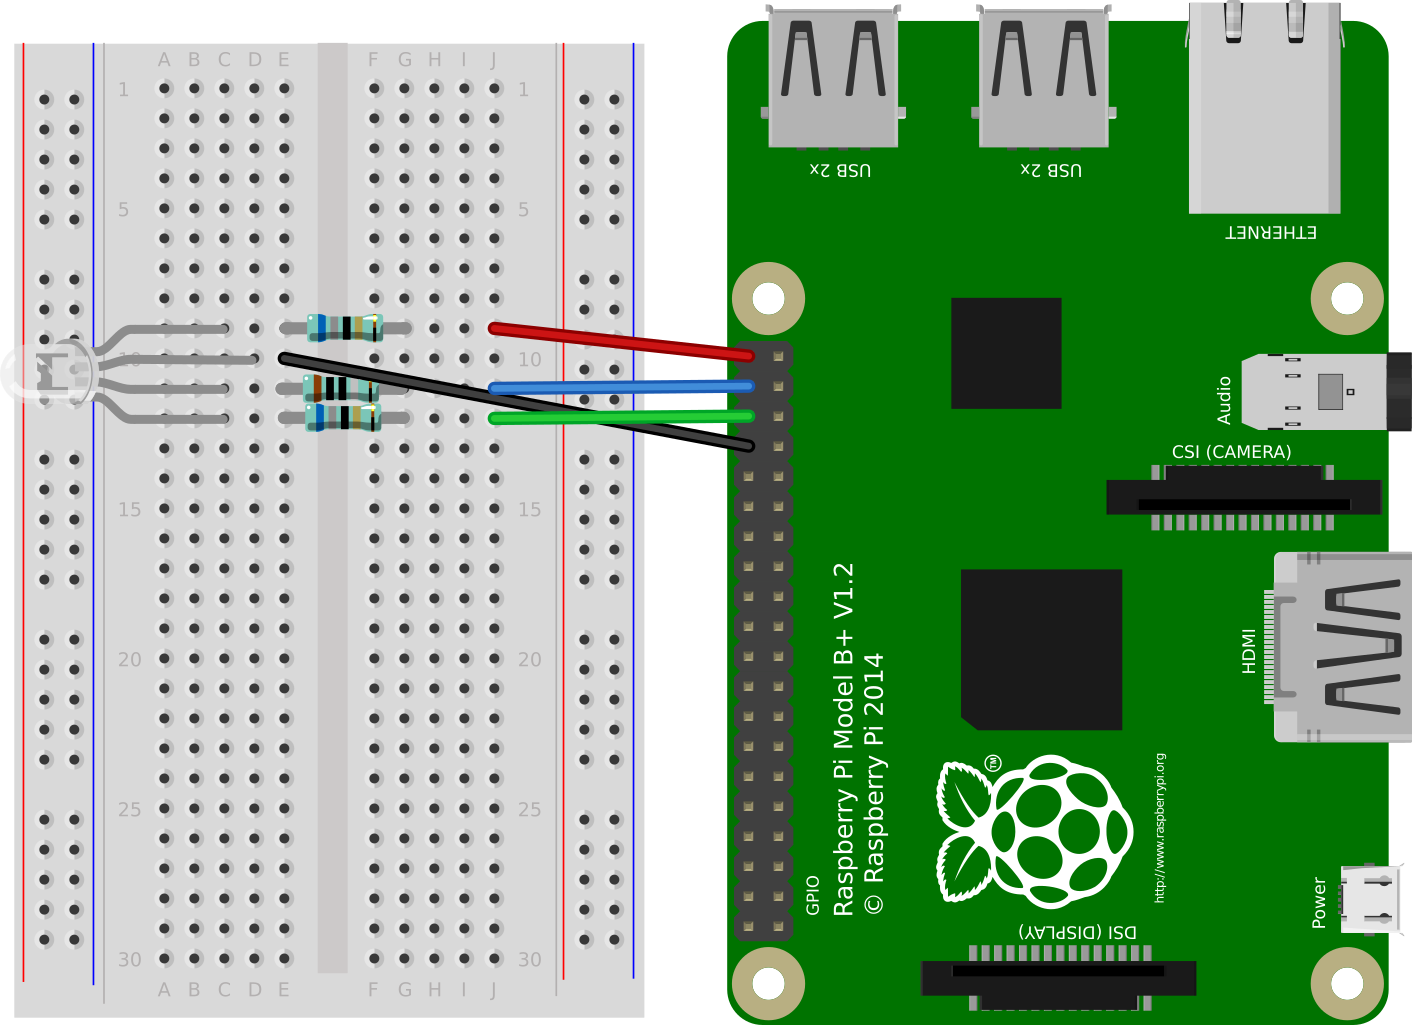
\includegraphics[width=0.7\linewidth]{McrRaspJam/015_GPIOZero/3_rgb/2}
	\end{center}
	
	Note that because the blue LED has a much higher forward voltage ($3.3 V$) we use a different $1 \Omega$ resistor for that pin.
	
	\subsection*{Programming the RGB LED}
	
		You can program the RGB LED as three separate LEDs in your program---you could try running your traffic light program using the RGB LED---however, GPIO Zero offers a separate RGBLED type, which makes colour mixing much easier.
		
		You can use the following program to test your RGB LED.
		
		\lstinputlisting[style=Python]{McrRaspJam/015_GPIOZero/3_rgb/rgb.py}
		
		If you're up for a challenge: Reading the online documentation for the function \texttt{pulse()}, try writing a program which cycles through every colour in the rainbow.